\subsection{User interface overview}
	When started, \PQUEUE\ shows its main window
	as depicted in figure \ref{pqueue:main_window}.

	\begin{figure}[!ht]
	\centering
	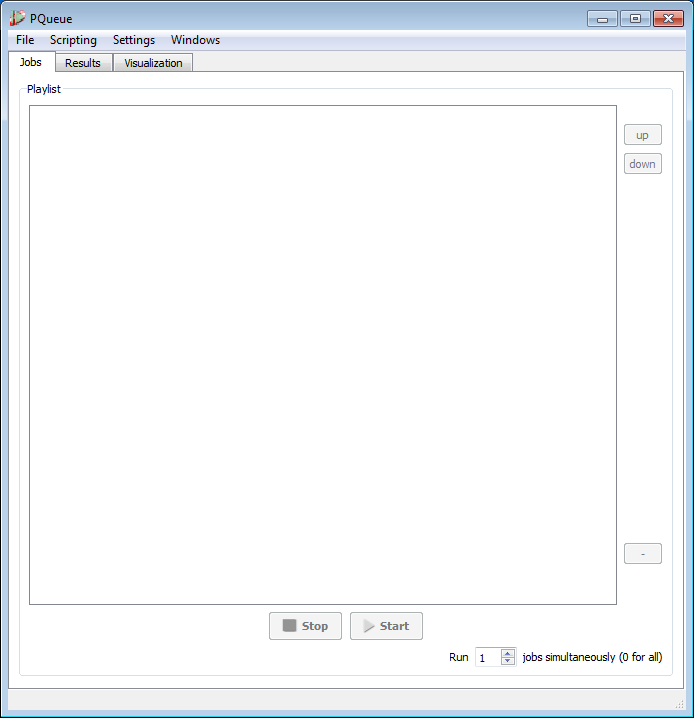
\includegraphics[width=0.75\textwidth]{Screenshots/PQueue/main_window.png}
	\caption{\PQUEUE's main window.}
	\label{pqueue:main_window}
	\end{figure}

	It consists of three tabs, named \textit{Jobs}, \textit{Results} and \textit{Visualization},
	from which the first is displayed in the screenshot.
	Each tab is discussed in detail in the sections \ref{pqueue:running_jobs} (\nameref{pqueue:running_jobs}),
	\ref{pqueue:results} (\nameref{pqueue:results}) and
	\ref{pqueue:visualization} (\nameref{pqueue:visualization}) respectively.

	There are several additional docking windows that are accessible through the application's menu \textbf{Windows}.
	These windows may be moved, resized and docked to any of the main window's edge
	or even detached from the main window.
	Figure \ref{pqueue:all_dock_widgets} shows an example.

	\begin{figure}[!ht]
	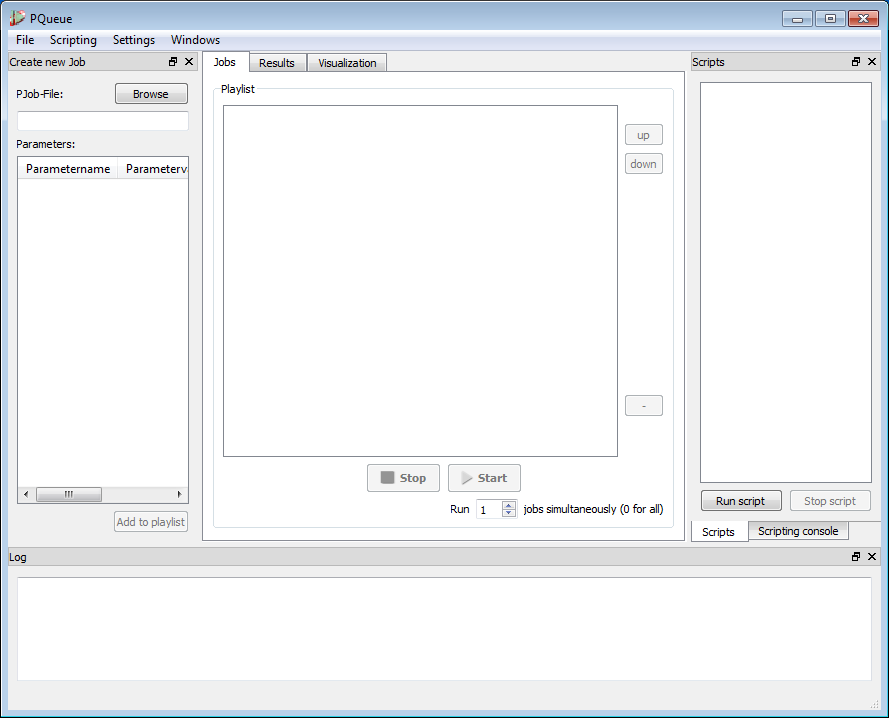
\includegraphics[width=\textwidth]{Screenshots/PQueue/all_dock_widgets.png}
	\caption{All of \PQUEUE's dock windows.}
	\label{pqueue:all_dock_widgets}
	\end{figure}

	The \textit{log} window displays a log showing all \PQUEUE\ events.
	The \textit{create job} window is used to add a job to the playlist by stating a \PJOB\ file
	and providing parameters.
	The \textit{scripting console} window allows the execution of single statements within \PQUEUE's
	script engine and shows script output and results.
	Whole script files are managed and run via the \textit{scripts} window.


\subsection{Settings}
\label{pqueue:settings}

	Also, there is a \textit{settings} window,
	which is accessible via \textbf{Settings} -\textgreater \textbf{Edit...} within the applications main menu.

	\begin{figure}[!ht]
	\centering
	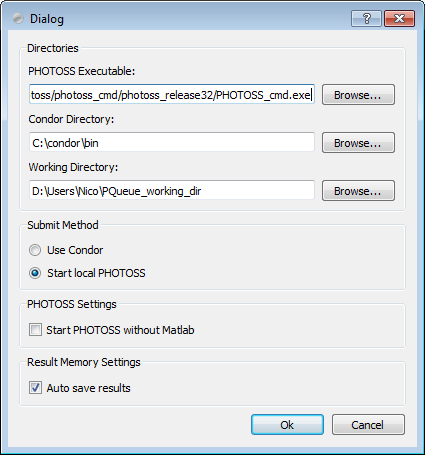
\includegraphics[width=0.6\textwidth]{Screenshots/PQueue/settings.png}
	\caption{\PQUEUE's settings windows.}
	\label{pqueue:settings_window}
	\end{figure}
	
	In order to be able to utilize \PHO\ and \Condor,
	\PQUEUE\ needs to know the directories where these applications are installed in.
	For \PHO\ this should be the directory where the file \textit{PHOTOSS\_cmd.exe} resides.
	For \Condor\ it's the directory containing \Condor's binaries, for example \textit{condor\_submit.exe}.
	
	When running a job,
	\PQUEUE\ creates a temporary directory in which a temporary copy of the \PJOB\ file
	and the \Condor\ log files are stored.
	These directories are created in \PQUEUE's \textit{working directory}
	which is set via the setting's dialog third text field.
	
	Wether to execute a job locally, i.e. on the same machine \PQUEUE\ is running on,
	or to use \Condor\ (i.e. \textit{condor\_submit}) to submit jobs to the \Condor\ pool,
	is set with the \textit{submit method} setting.
	
	If you are using \Condor\ and your pool is heterogenous in terms of \MAT\ installations,
	i.e. you can't assume to have a working \MAT\ installation on every machine,
	you may run into problems if \PHO\ is trying to initialize \MAT\ from the context of a \Condor\ job.
	Therefore \PHO\ provides the command line switch \textit{--matlab} to set a specific \MAT\ version
	or to deactivate \MAT\ support altogether.
	To make \PQUEUE\ start \PHO\ without \MAT\ support,
	activate the setting \textit{Start PHOTOSS without Matlab}.





\subsection{Adding and running jobs}
\label{pqueue:running_jobs}

Within the context of \PQUEUE,
a \textit{job} is a \PJOB\ file \textbf{and} values for all of the file's parameters.
So, in order to add a job to the queue,
you have to choose an already existing \PJOB\ file and provide values for it's parameters.
This is done via the \textit{create job} window as shown in figure \ref{pqueue:adding_jobs}.

\begin{figure}[!ht]
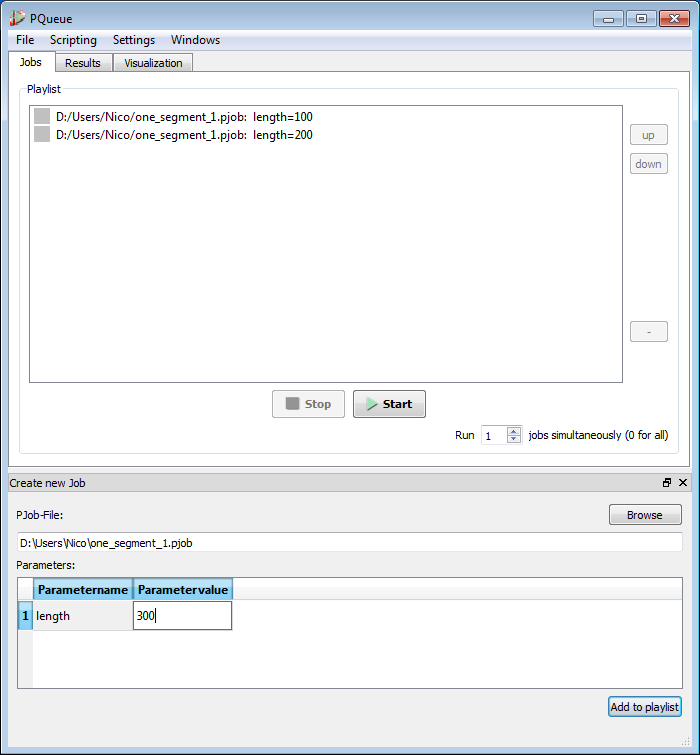
\includegraphics[width=\textwidth]{Screenshots/PQueue/adding_jobs.png}
\caption{Adding jobs to the queue.}
\label{pqueue:adding_jobs}
\end{figure}

As soon as a path to a valid \PJOB\ file is given,
its parameters are read and shown in the table view below.
The values in the column \textit{Parametervalue} can be edited after double clicking.
Pressing the \textit{Add to playlist} button adds the \PJOB\ to the queue with the parameter values currently set in the table view.\bb


Jobs can be arranged within the queue by using the \textit{up} and \textit{down} buttons after selecting a job.
The \textit{-} button removes the selected jobs from the queue.
When \textit{Start} is pressed (or a script triggers execution),
jobs are processed sequentially from top to bottom.
In order to utilize the resources at hand
but avoid overhead,
you might want \PQUEUE\ to execute as many jobs in parallel as there are cores on your machine,
or in the pool respectively.
Therefore the number of jobs executed simultaneously can be set with the spin box in the lower right corner.

\subsubsection{Job states}

During execution, jobs change their state from \textit{queued} over \textit{submitted} and \textit{running}
to \textit{finished} ultimately.
The colored square to the left of the job's file path represents the state.
Gray is for \textit{queued} which means the job is added to the queue but execution was not triggered yet.
Yellow (\textit{submitted}) means the job was submitted to the \Condor\ pool
but no machine was matched yet.
(When executing locally, this state is omitted.)
Dark green means the job is \textit{running} at the moment.
When it's \textit{finished} the square's color changes to light green.





\subsection{Results}
\label{pqueue:results}

Automatically running multiple jobs in sequence
would not make sense if the jobs did not produce results
and also if these results were not collected and saved by \PQUEUE.
Therefore \PQUEUE\ incorporates a result memory
which, in essence, holds a mapping from parameter values to result values
for every \PJOB\ file that was executed.

\begin{figure}[!ht]
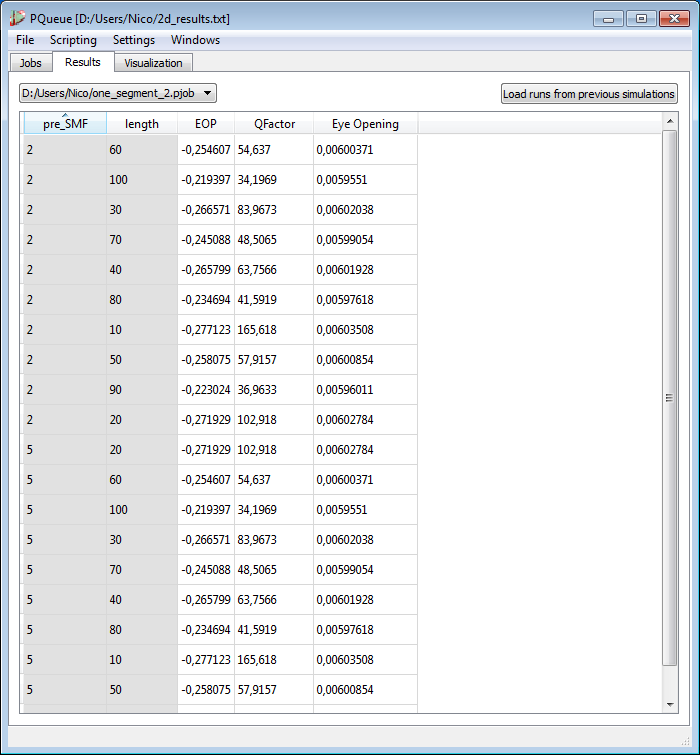
\includegraphics[width=\textwidth]{Screenshots/PQueue/results.png}
\caption{\PQUEUE's result view.}
\label{pqueue:results}
\end{figure}

The main window's second tab shows the result memory by utilizing a table view.
Results are viewed by \PJOB\ file.
That means, first you have to choose the \PJOB\ file for which to view results
by using the combo box in the top left corner.
Now the table view below shows all calculated parameter combinations with their according results
for the selected \PJOB\ file.
Parameter columns are marked gray.
Lines can be sorted by clicking on any column's header.

\subsubsection{Loading and Saving results}
After launching \PQUEUE, its result memory is empty.
When executing jobs,
\PQUEUE\ automatically reads new results from the \PJOB\ file into the result memory.
You might want to save results to a file for further processing.
(Although all results are already saved within the \PJOB\ file's run directories.)
\PQUEUE\ writes and reads its result memory to CSV \footnote{\textit{comma separated values}, also called \textit{flat file}} files.
Writing is triggered via \textbf{File} -\textgreater \textbf{Save results} or \textbf{File} -\textgreater \textbf{Save results as...} and choosing a file path.
The created file contains all information stored in the result memory,
so that \PQUEUE\ is able to restore its result memory by importing a formerly exported file
(via \textbf{File} -\textgreater \textbf{Load results...}).

As mentioned above,
\PJOB\ files contain run directories for every execution.
Since the parameter combination is stored within the run directory,
there already is a result memory in every \PJOB\ file.
Via \textbf{File} -\textgreater \textbf{Import from PJob...},
\PQUEUE\ is able to import all results stored in a \PJOB\ file

If the setting \textit{Auto save results} is activated,
\PQUEUE\ will save the result memory every time new results are received.
For this to work, results must have been saved once before or loaded from file,
so that \PQUEUE\ knows which file to write to.


\subsubsection{Result memory file format}
Exported result memory files can be used to process results with 3rd party tools like Excel for example.
These files store one parameter combination per line with parameter and result values separated by tabulators (\textit{\textbackslash t}).

The first lines, beginning with \textit{\%}, are header files conveying additional information.
For a result space containing results for \textit{n} different \PJOB\ files,
there are \textit{n+1} header lines,
one for each \PJOB\ file and one line (the last header line) stating the column's names separated by tabulators.

The \textit{n} \PJOB\ file header lines contain the \PJOB\ file's path,
its parameter list and its result list.
Parameters are separated from results by two tabulators
to make it possible to distinguish parameters and results without having to know the \PJOB\ file. 



\subsection{Result visualization}
\label{pqueue:visualization}

As long as only one parameter is varied,
the result table described above may be sufficient to view the results.
Since \PQUEUE\ enables the \PHO\ user to conduct huge parameter variations,
possibly variating a huge number of parameters,
it also provides means of visualizing and exploring multidimensional result spaces.

\begin{figure}[!ht]
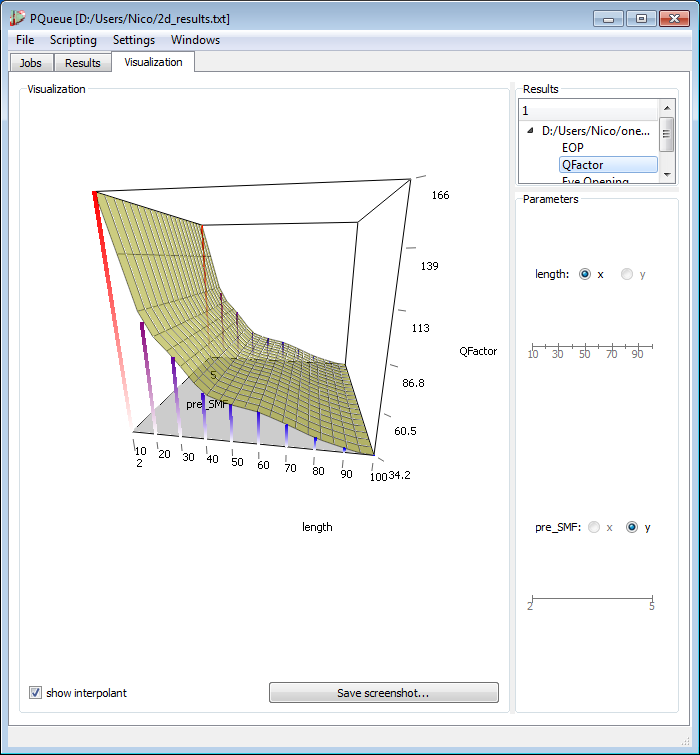
\includegraphics[width=\textwidth]{Screenshots/PQueue/visualization.png}
\caption{\PQUEUE's result visualization.}
\label{pqueue:visualization_screenshot}
\end{figure}

The main window's third tab shows a 3D view visualizing data stored in the result memory.
On the top right, there is a tree view showing all results sorted by \PJOB\ files.
Selecting a result in this tree view determines which result is visualized within the 3D area.
Below the results tree view are radio buttons and sliders for each of the selected \PJOB\ file's parameters.


\subsubsection{3D view}
The 3D view always shows a box for guidance.
When a result is selected in the results tree view,
it also shows the stored values of this result.
Every result value is represented by a colored pillar.
Both color and height correspond to the result's value.
Position of the pillar corresponds to the parameter combination for which
this result value was calculated.
If there are only two parameters this seems natural.
For more parameters,
two have to be chosen to represent the dimensions constituting the box's floor.
The 3D view then shows a two-dimensional intersection of the multidimensional result space.
(See section \nameref{pqueue:vis:parameter} below.)\bb

The view's angle and zoom can be changed by mouse interaction.
Moving the mouse cursor over the 3D view while holding any mouse button down
changes the views angle of sight.
Using the mouse wheel while the mouse cursor is over the view changes the zoom factor.\bb

The view can be saved to an image file (BMP or PNG) by clicking the \textit{Save screenshot...} button
and providing a file path to save to.

\subsubsection{Interpolation function}
\label{pqueue:interpolation_function}
For conveniently exploring a sparse sampled result space,
a multidimensional interpolation function was implemented
that can be added to the 3D view by activating the checkbox \textit{show interpolation function} below the view.

The interpolation method used here is the \textit{Hardy Multi Quadric} which is a \textit{scattered data} interpolation function.
The function is defined by
\textbf{\begin{equation}
	f(x)= \sum_{i=1}^{N} \alpha_{i} R(d_{i}(x)),
\end{equation}}
with $\alpha_{i}$ being the interpolation coefficients that have to be determined
depending on the known data vectors and
$d_i(x)$ being the distance to the $i$-th data vector.
$R(r_i)$ is defined as follows:
\begin{equation}
	R(r_{i}) = (r_{i}^{2} + R_{i}^{2})^{\frac{\mu_{i}}{2}},
	\;
	\mu \neq 0,
\end{equation}
We set $\mu_i = 0.5$ and $R_{i}=0$ for all $i$, simplifying the interpolation function to
\textbf{\begin{equation}
	f(x)= \sum_{i=1}^{N} \alpha_{i} \sqrt{d_{i}(x)}.
\end{equation}}
$\alpha$-coefficients are determined by solving
\begin{equation}
	\min_{\vec{\alpha}} \left\|
	\left( 
	\begin {array} {cccc}
	R(d_{1}(x_{1})) & R(d_{2}(x_{1})) & \dots & R(d_{n}(x_{1})) \\
	R(d_{1}(x_{2})) & R(d_{2}(x_{2})) & \dots & R(d_{n}(x_{2})) \\
	\vdots & \vdots & \vdots & \vdots \\
	R(d_{1}(x_{n})) & R(d_{2}(x_{n})) & \dots & R(d_{n}(x_{n})) \\
	\end {array}
	\right)
	\left( 
	\begin {array} {c}
	\alpha_{1} \\
	\alpha_{2} \\
	\vdots \\
	\alpha_{n}
	\end {array}
	\right)
	-
	\left( 
	\begin {array} {c}
	f_{1} \\
	f_{2} \\
	\vdots \\
	f_{n}
	\end {array}
	\right)
	\right\|.
\end{equation}



\subsubsection{Parameters}
\label{pqueue:vis:parameter}
On the right side of the \textit{Visualization} tab, below the results tree view,
is a list of the selected \PJOB\ file's parameters.
For every parameter, there are two radio buttons reading \textit{x} and \textit{y} respectively
and a slider below.
These widgets control which part of the multidimensional result space is shown within the 3D view.

By clicking the appropriate radio buttons,
one parameter is set to constitute the \textit{x}-axis and another to constitute the \textit{y}-axis.
For these two parameters, the sliders are disabled, because all of their parameter values are shown.
For the remaining parameters, a distinct value has to be set for which to show the results.
This is done by setting the remaining sliders to the appropriate values.
Every parameter combination (i.e. combination of slider positions) will show a different part of the result space.





\subsection{PQueue scripts}
Much like \PHO, \PQUEUE\ incorporates a script engine and therefore can be controlled programmatically.
Jobs can be submitted and results can be evaluated from within a script.
Basically, everything the user could do manually can be done with a script, and even more.
One particular use case for this is the optimization of \PHO\ simulations.
With \PQUEUE\ scripts, parameter combinations that are to be calculated next
can be chosen depending on newly received results.
The section \textit{\nameref{pqueue:scripts:built-in}} below discusses this topic and shows an example.
But first, section \textit{\nameref{pqueue:scripts:executing}} shows how to load and run scripts
and section \textit{\nameref{pqueue:scripts:tutorial}} introduces \PQUEUE\ scripts thoroughly.

\subsubsection{Executing scripts}
\label{pqueue:scripts:executing}
The easiest way to execute script code is by using the script console (\textbf{Windows} -\textgreater \textbf{Show script console}).
The edit line at the bottom of this window accepts script code that gets executed immediately after hitting return.
Output generated by any script code is shown in the field above that edit line.\bb

To load a script file into \PQUEUE's memory, choose \textbf{Scripting} -\textgreater \textbf{Load script from file...} from the menu.
The script is then shown in the \textit{Scripts} window which shows all loaded scripts.
Any loaded script can be executed by selecting it and pressing the \textit{Run script} button.
As long as a script is running, a progress bar is displayed on the \textit{Scripts} window.\bb

There are also built-in scripts that are accessible via \textbf{Scripting} -\textgreater \textbf{Built-in scripts}.
Selecting one of these will execute the script immediately.



\subsubsection{Tutorial}
\label{pqueue:scripts:tutorial}
\PQUEUE's script engine implements an ECMAScript dialect.
It makes \PQUEUE's runtime objects accessible within the script context.
In the following, it is assumed that you are familiar with ECMAScript (i.e. JavaScript).\bb

\PQUEUE\ adds global objects and functions to the script context.
The job queue, \PQUEUE's main data structure, can be accessed via the Object \textit{PQueue}.
To start execution of the queue, you can call its \textit{start()} method.
\lstset{basicstyle=\color{black},backgroundcolor=\color{gray}, language=PQueueScript}
\begin{lstlisting}
PQueue.start(1);
print("Queue started!");
\end{lstlisting}
The \textit{start()} method's argument sets \PQUEUE\ to start only one job at a time.
\textit{print()} produces output that is shown in the script console.\bb

Adding jobs to the queue is done by first creating a job object
and second calling \textit{addJob} on the \textit{PQueue} object.
\begin{lstlisting}
var parameters = {"length": 100, "pre_SMF": 5, "pre_DCF": 4};
var j = new Job("D:\\Users\\Nico\\one_segment.pjob", parameters);
PQueue.addJob(j);
print("Added job to the queue");
\end{lstlisting}
The \textit{Job} constructor takes two arguments.
First a string stating the \PJOB\ file's path
and second an object that holds a property for every of the \PJOB\ file's parameters.
In the example above, this object is constructed using ECMAScript's object literal syntax in line 1.
Now, this makes it easy to create a queue variating one of the \PJOB\ file's parameters.
\begin{lstlisting}
if(PQueue.isRunning()) PQueue.stop();
for(length = 10; length<=100; length += 10){
	var parameters = {"length": length, "pre_SMF": 5, "pre_DCF": 4};
	var j = new Job("D:\\Users\\Nico\\one_segment.pjob", parameters);
	PQueue.addJob(j);
}
\end{lstlisting}\bb

If you want to do complex calculations between job executions,
waiting for a job to finish my be a prerequisite.
Therefore job objects implement the \textit{waitUntilFinished()} method.
This method blocks script execution until the job on which it's called is finished.
The following listing shows how to use this method to wait until all previously created jobs finished execution.
\begin{lstlisting}
var parameters = {"length": 5, "pre_SMF": 5, "pre_DCF": 4};
var jobs = new Array();
for(length = 10; length<=100; length += 10){
	parameters.length = length;
	var j = new Job("D:\\Users\\Nico\\one_segment.pjob", parameters);
	PQueue.addJob(j);
	jobs.push(j);
}
PQueue.start();
for(var i in jobs){
	jobs[i].waitUntilFinished();
}
print("All jobs are finished!");
\end{lstlisting}



\subsubsection{Built-in scripts}
\label{pqueue:scripts:built-in}

\newpage
\subsubsection{Function reference}

\begin{itemize}
	\item \textbf{PQueue} - object
	\begin{itemize}
		\item \textbf{addJob(job)} - function\\
		takes a job object (created with \textit{new Job(...)}) and adds it to the queue.
		\item \textbf{removeJob(job)} - function\\
		takes a job object (created with \textit{new Job(...)}) and removes it from the queue.
		\item \textbf{start(jobs\_simultaneously)} - function
		\item \textbf{stop()} - function 
		\item \textbf{isRunning()} - bool function
	\end{itemize}
	
	\item \textbf{Job(pjob\_file, paramters)} - constructor\\
	Creates a job object and takes two arguments. First the path to the \PJOB\ file.
	Second an object that holds a property for every of the \PJOB\ file's parameters.
	I.e. if the \PJOB\ file has one parameter \textit{length}
	the given object needs to have a property called \textit{length}.
	ECMAScript literal syntax for objects is \textit{ \{'length': 5\}}.
	
	Job objects have only one function:
	\begin{itemize}
		\item \textbf{waitUntilFinished()} - function\\
		Blocks script execution until the job, on which this function was called, is finished.
	\end{itemize}
	
	\item \textbf{HardyMQ(pjob\_file, result)} - constructor\\
	Creates a Hardy Multi Quadric interpolation function (see section \ref{pqueue:interpolation_function} for details)
	and takes two parameters.
	First a path to a \PJOB\ file for which results are present in the result memory
	and second the name of one of the \PJOB\ file's result.
	The created interpolation function uses the result values determined by these parameters as data vectors.
	
	Created objects implement the following functions:
	\begin{itemize}
		\item \textbf{getValue(parameters)} - function\\
		Takes an object as argument that holds a property for every parameter of the \PJOB\ file
		this interpolation function was created for.
		(I.e. \textit{getValue(\{'length':100, 'power':5\})})
		Returns the interpolation function evaluated at the given parameter combination.
		
		\item \textbf{findMinimum()} - function\\
		Tries to find the interpolation function's minimum by using simulated annealing.
		
		\item \textbf{findMaximum()} - function\\
		Tries to find the interpolation function's maximum by suing simulated annealing.
	\end{itemize}
	
	\item \textbf{print(string)} - function\\
	Prints the given string to the script console's output window.
	
	\item \textbf{userInput()} - function\\
	
	
	\item \textbf{readParametersFromPJOBFile(file\_path)} - function\\
	Opens the given \PJOB\ file, reads its parameter definitions and returns an object
	that holds a property for every read parameter.
	The properties are also objects and their names correspond to the parameters' names.
	The sub-objects have at least the property \textit{defaultValue} and, if the parameter definitions includes this information,
	the properties \textit{minValue} and \textit{maxValue}.
	Example:
	\begin{lstlisting}
	var pjobParameters = readParametersFromPJOBFile("D:\\my_job.pjob");
	for(var parameter_name in pjobParameters){
		print("Found parameter: " + parameter_name + " with default value: " + pjobParameters[parameter_name].defaultValue);
	}
	\end{lstlisting}
	
	
	\item \textbf{isExistingFile(file\_path)} - function\\
	Returns \textit{true} if the given file exists, false otherwise.
	
	\item \textbf{saveResults(file\_path)} - function\\
	Saves the result memory to the given file.
	
	
\end{itemize}


